
%% bare_conf.tex
%% V1.4b
%% 2015/08/26
%% by Michael Shell
%% See:
%% http://www.michaelshell.org/
%% for current contact information.
%%
%% This is a skeleton file demonstrating the use of IEEEtran.cls
%% (requires IEEEtran.cls version 1.8b or later) with an IEEE
%% conference paper.
%%
%% Support sites:
%% http://www.michaelshell.org/tex/ieeetran/
%% http://www.ctan.org/pkg/ieeetran
%% and
%% http://www.ieee.org/

%%*************************************************************************
%% Legal Notice:
%% This code is offered as-is without any warranty either expressed or
%% implied; without even the implied warranty of MERCHANTABILITY or
%% FITNESS FOR A PARTICULAR PURPOSE! 
%% User assumes all risk.
%% In no event shall the IEEE or any contributor to this code be liable for
%% any damages or losses, including, but not limited to, incidental,
%% consequential, or any other damages, resulting from the use or misuse
%% of any information contained here.
%%
%% All comments are the opinions of their respective authors and are not
%% necessarily endorsed by the IEEE.
%%
%% This work is distributed under the LaTeX Project Public License (LPPL)
%% ( http://www.latex-project.org/ ) version 1.3, and may be freely used,
%% distributed and modified. A copy of the LPPL, version 1.3, is included
%% in the base LaTeX documentation of all distributions of LaTeX released
%% 2003/12/01 or later.
%% Retain all contribution notices and credits.
%% ** Modified files should be clearly indicated as such, including  **
%% ** renaming them and changing author support contact information. **
%%*************************************************************************


% *** Authors should verify (and, if needed, correct) their LaTeX system  ***
% *** with the testflow diagnostic prior to trusting their LaTeX platform ***
% *** with production work. The IEEE's font choices and paper sizes can   ***
% *** trigger bugs that do not appear when using other class files.       ***
% The testflow support page is at:
% http://www.michaelshell.org/tex/testflow/



\documentclass[10pt,conference,compsoc]{IEEEtran}
% Some Computer Society conferences also require the compsoc mode option,
% but others use the standard conference format.
%
% If IEEEtran.cls has not been installed into the LaTeX system files,
% manually specify the path to it like:
% \documentclass[conference]{../sty/IEEEtran}

\usepackage{cite}
\usepackage[utf8]{inputenc} %para introdução de caracteres especiais
\usepackage[english]{babel}
\usepackage{tikz}
\usepackage{scalefnt}
\usepackage{comment} 
\usepackage{graphicx}
\usepackage{url}
\usepackage{xspace}
\usepackage{commath}

\begin{document}

\newcommand{\robobo}{\texttt{Robobo}\xspace}
\newcommand{\ros}{\texttt{ROS}\xspace}

\title{Robobo Line Follower}

% author names and affiliations
% use a multiple column layout for up to three different
% affiliations
\author{\IEEEauthorblockN{\^{A}ngela Cardoso}
\IEEEauthorblockA{Faculdade de Engenharia da Universidade do Porto\\
Rua Dr. Roberto Frias, 4200-465 Porto, Portugal\\
Email: angela.cardoso@fe.up.pt}}

% make the title area
\maketitle

% As a general rule, do not put math, special symbols or citations
% in the abstract
\begin{abstract}
As a form of testing and learning the \ros framework implementation in the smartphone robot \robobo, a line following program was designed and implemented. The line is sensed with the camera on the phone, whose image is processed using OpenCV. A colored line on white background map was used to test the behavior of the robot and to manually tune the PID constants. The results show that the robot manages to follow the line while maintaining stability. However, due to the lack of quality from the camera image, the linear velocity of the robot must be low. Also, better PID constants can very likely be obtained through a more sophisticated tunning.
\end{abstract}

\begin{IEEEkeywords}
Mobile robots, Reactive robots, Image Processing, PID control, Smartphone robots.
\end{IEEEkeywords}

%%%%%%%%%%%%%%%%
% INTRODUCTION %
%%%%%%%%%%%%%%%%
\section{Introduction}

\robobo~\cite{Robobo} is an educational robot developed by Mytechia. In terms of hardware it consists of a wheeled robotic base where an \texttt{Android} smartphone must be placed. The phone uses Bluetooth to communicate with the base and Wi-Fi to communicate with a computer, which is used to program the behavior of the robot.

Currently, there are three ways to program \robobo~\cite{Robobo_Programming}. The simplest is block programming, which uses the \robobo \texttt{Android} application on the phone and a \texttt{ScratchX}~\cite{Scratch} extension on a computer. One can also use native programming, with the \texttt{Java} language and the \texttt{Robobo Framework}. Finally, and of most interest to us, \robobo can be programmed with \ros~\cite{ROS,AGITR}, using the \texttt{Android} application \texttt{Robobo Developer}. This application creates a \ros master node at the phone, to which a computer running \ros and using a set of defined custom messages connects, in order to control the behavior of the robot.

In order to test and get acquainted with implementation of the \ros framework in \robobo, a simple reactive robot was implemented. It uses the camera in the smartphone to detect a line of a previously determined color (black, red, green or blue) and then attempts to follow that line indefinitely. 

The system developed barely makes use of memories or past experiences to inform its current decisions. However, in order to improve the robots stability, a Proportional–Integral–Derivative (PID) controller~\cite{PID_wiki,PID_line_follower} was used. This implies that at each moment, the previous error is known and used to compute the derivative term. A sum of all previous errors is also kept in the integral term. Therefore, this \robobo line follower is not purely reactive.

%%%%%%%%%%%%%%%%
% ARCHITECTURE %
%%%%%%%%%%%%%%%%
\section{Architecture}
\subsection{Robot Design and Camera Position}

As can be seen in Figure~\ref{fig:robobo}, the \robobo base possesses a smartphone holder. This holder is equipped with a pan movement, that allows it to rotate horizontally to the desired position, as well as a tilt movement, that can be use to rotate the phone vertically. 

\begin{figure}[thpb]
\centering

\includegraphics[scale=0.5]{img/robobo.png}
\caption{A \robobo robot.}
\label{fig:robobo}
\end{figure}

The base also has two wheels on the front and a plastic caster at the back, which allow it to rotate in place. In order to move the robot, the speed of each wheel must be defined, thus determining both its linear and angular velocities.

Because we want to move the robot forward, that is with the wheels in the front, and we want to use the camera on the back of the smartphone to detect the line to follow, the phone holder must be rotated clockwise, so that it stays approximately 180 degrees rotated from the position shown in Figure~\ref{fig:robobo}.

The vertical position of the phone should be around 130 degrees, a little lower then the position shown in Figure~\ref{fig:robobo}. This way, even though we will be processing only the portion of the image closest to the robot, that image is wider compared to a situation where the phone is lying down close to the base and the camera is directly facing the floor.

\subsection{Maps}
Two maps where used to test the line following \robobo. The first map is a simple curved black closed line in a white background, as shown in Figure~\ref{fig:map_black}.

\begin{figure}[thpb]
\centering
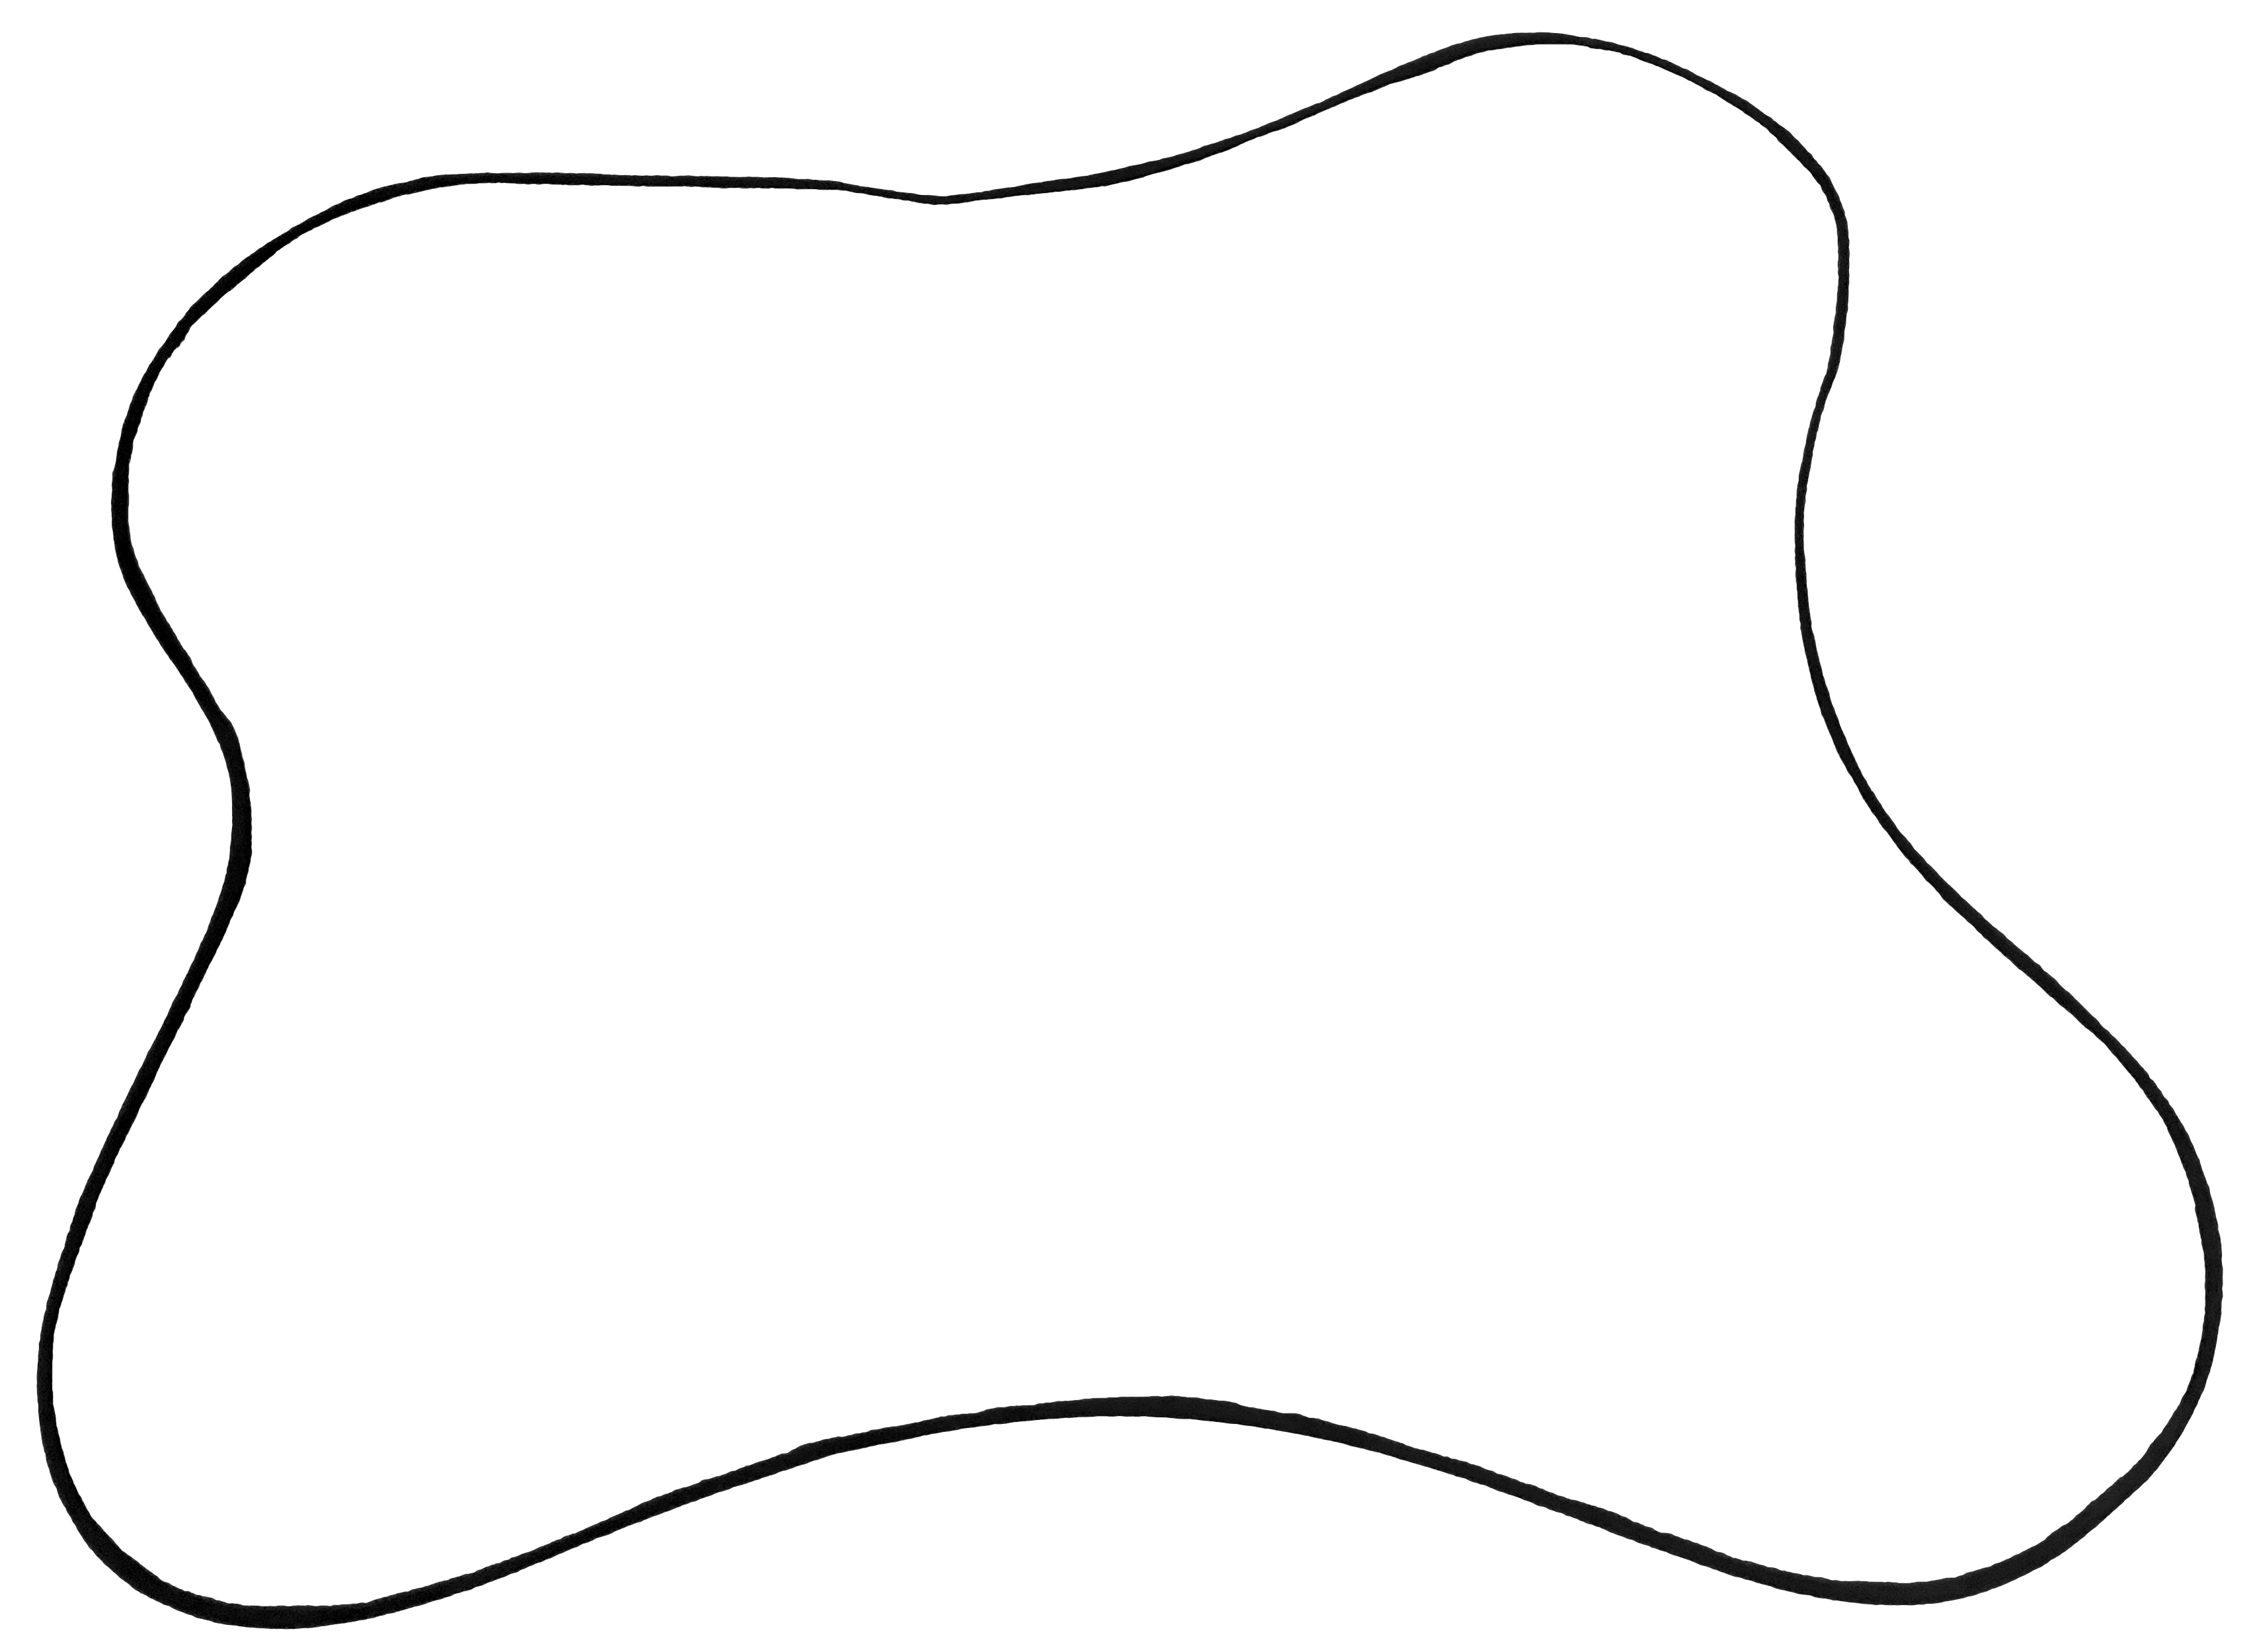
\includegraphics[scale=0.06]{img/map_black.png}
\caption{The black line test map.}
\label{fig:map_black}
\end{figure}

The second map, shown in Figure~\ref{fig:map_color}, has three lines in colors the red, green and blue. The color that the robot follows is chosen by setting a run time argument: 0 for black, 1 for red, 2 for green and 3 for blue. Of course these colors, except perhaps in the black case, must be calibrated, but that must be done manually in the program code. An interesting future development would be to add a color calibration mode, that could then be used to track any color the user may desire, as long as it can be sufficiently separated from the background and other possible colors on the map.

\begin{figure}[thpb]
\centering
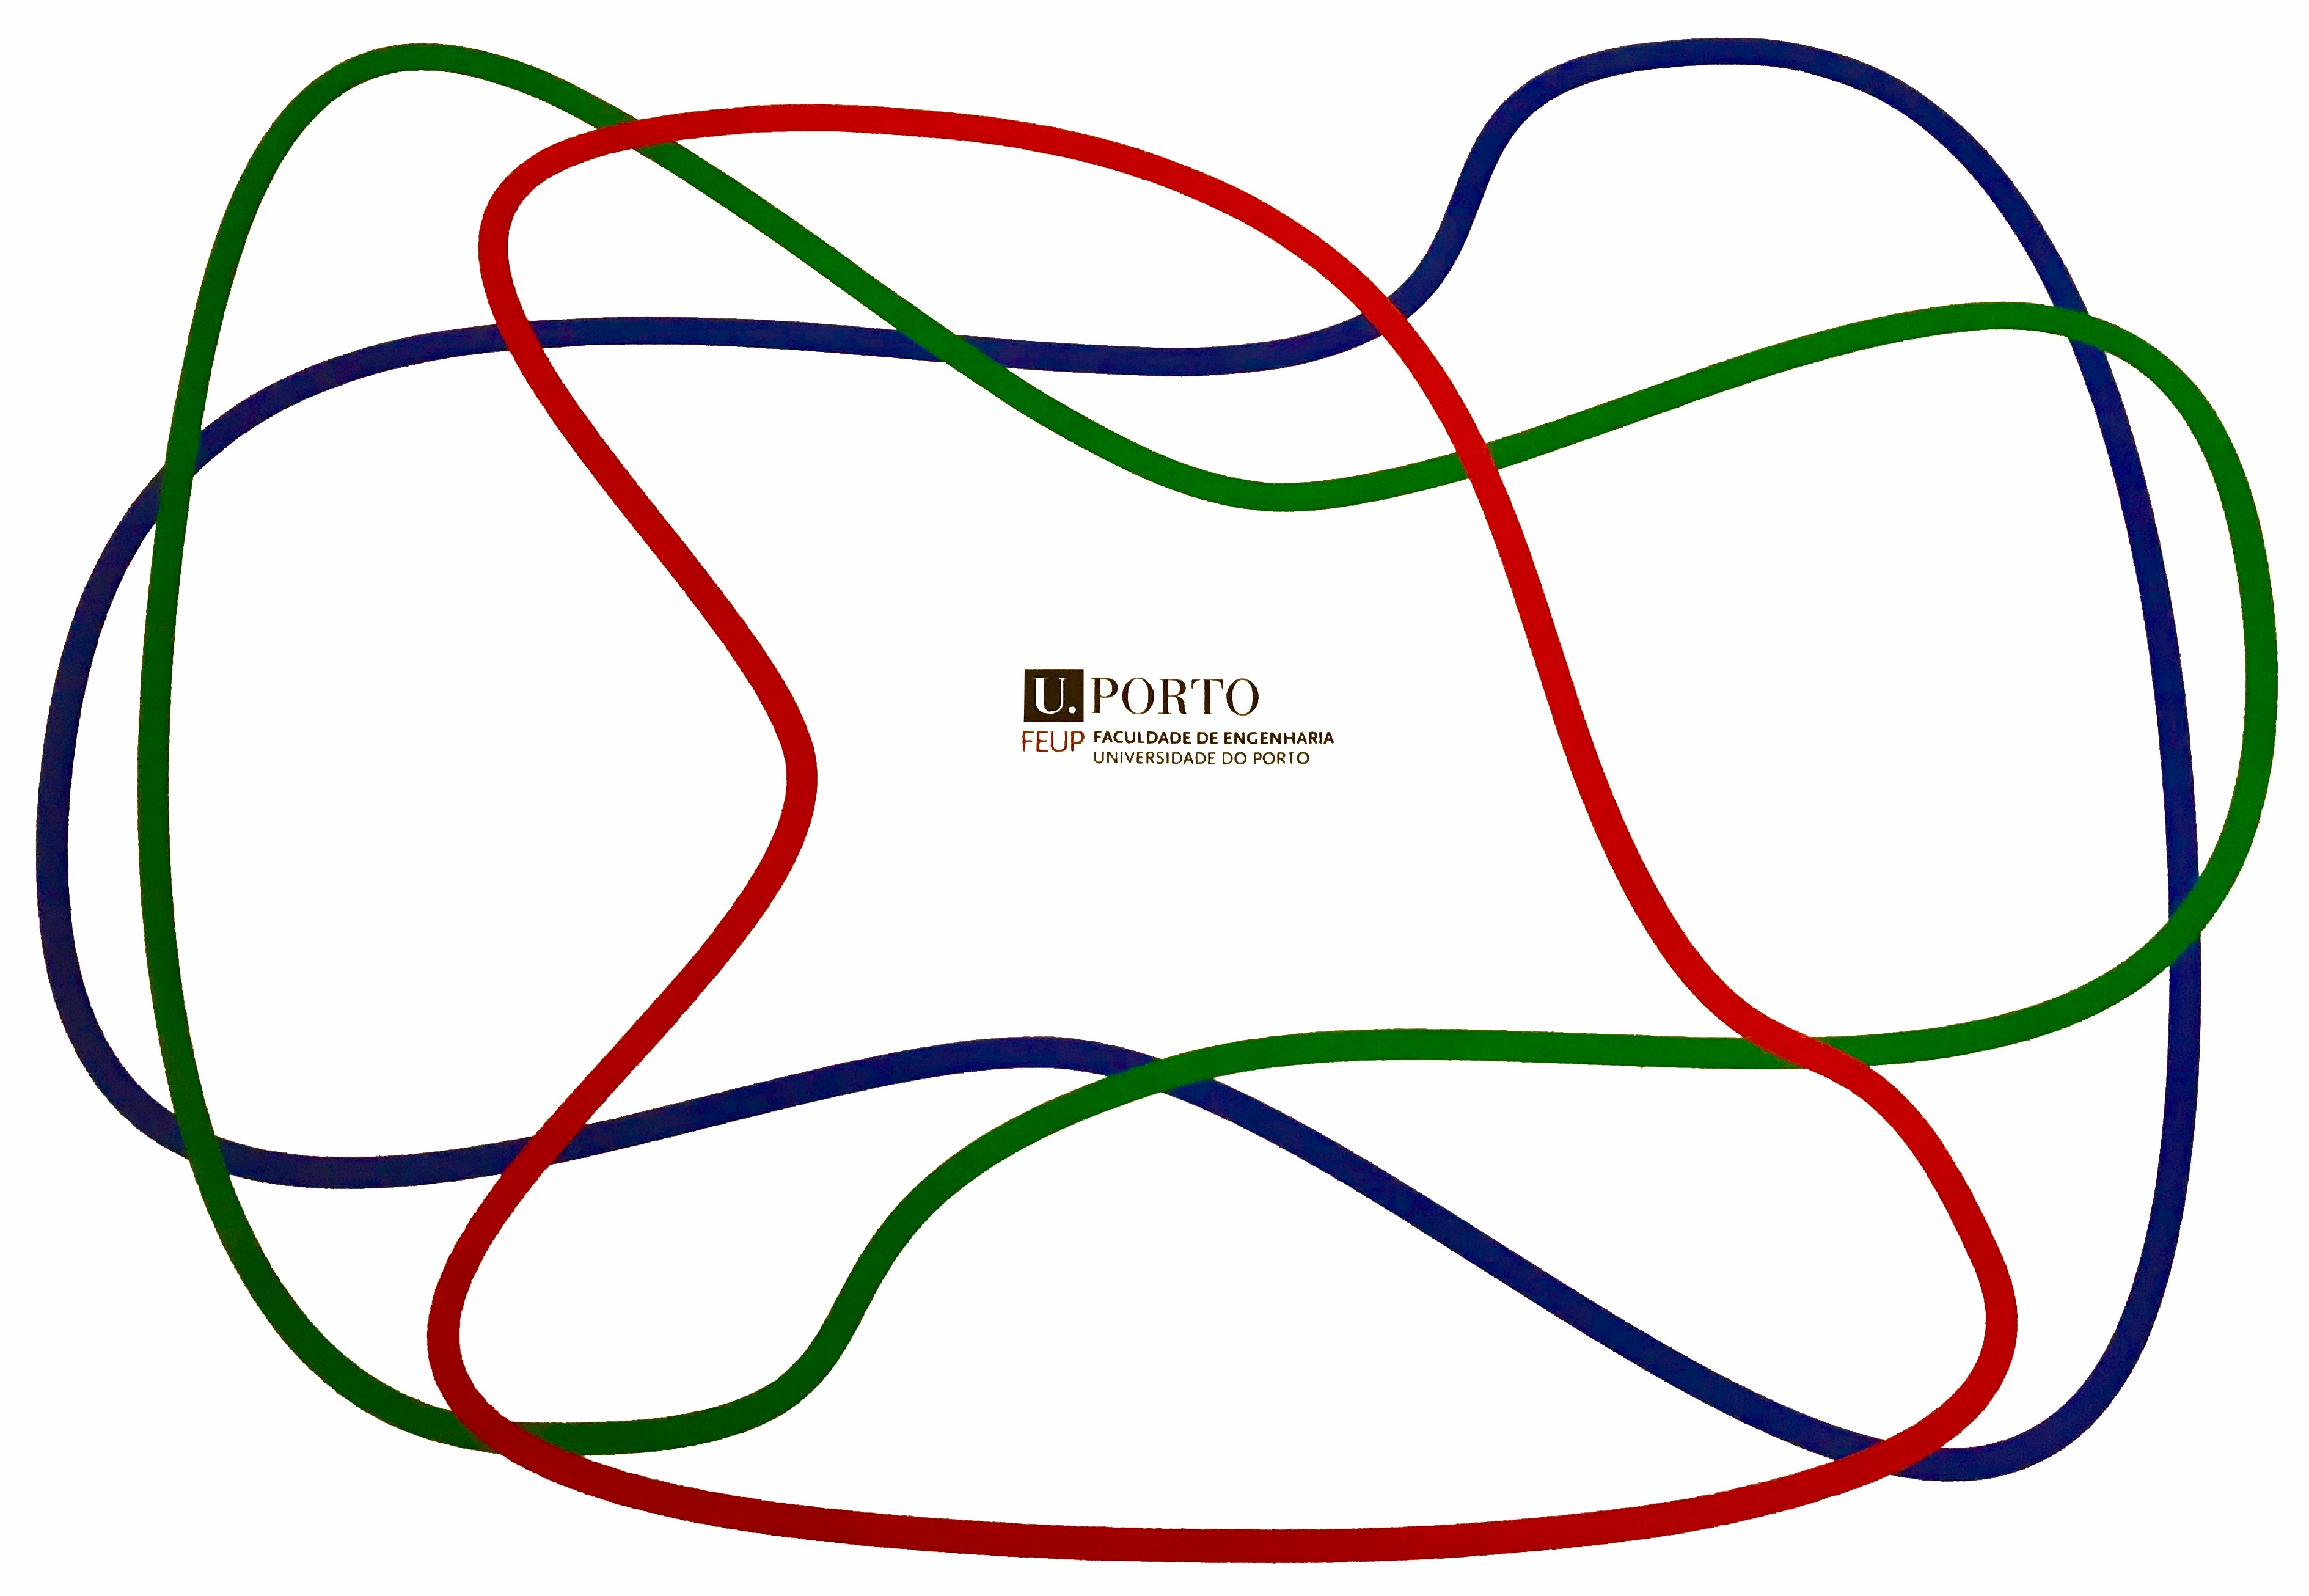
\includegraphics[scale=0.06]{img/map_color_final.jpg}
\caption{The colored lines test map.}
\label{fig:map_color}
\end{figure}

\subsection{Behavior Architecture}

The robot follows a timed finite state machine architecture, according to the diagram in Figure~\ref{fig:architecture}. It is timed, because whenever a new camera image is received, which is determined by the frequency of the spin function in \ros, the state the robot is in may change, and these are the only times that may happen.

\begin{figure}[thpb]
\centering
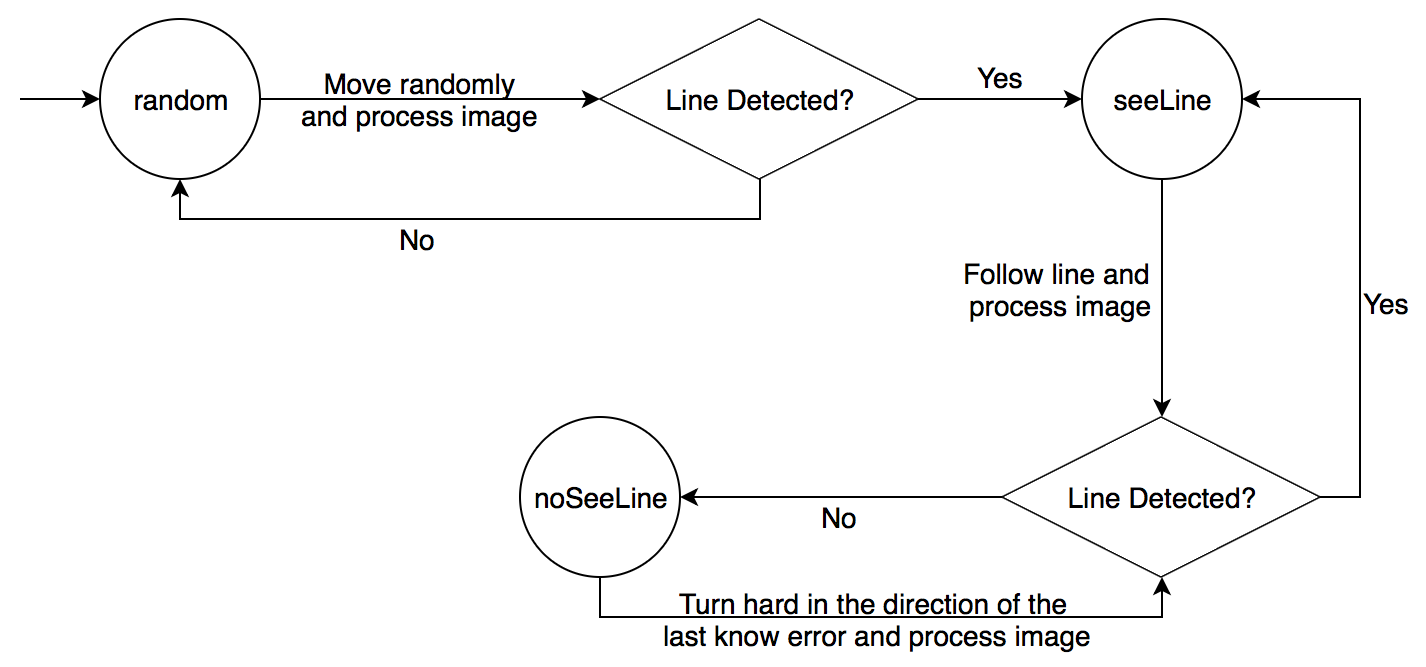
\includegraphics[scale=0.34]{img/architecture.png}
\caption{Timed finite state machine architecture.}
\label{fig:architecture}
\end{figure}

The initial state of the robot is \texttt{random}, because until the robot detects a line to follow, it will move randomly. At the first camera image received where a line is detected the new state will be \texttt{seeLine} and the robot will never go back to moving randomly. In fact, if it is not in the \texttt{seeLine} state, it will be in the \texttt{noSeeLine} state, meaning that the processing of the previous camera image did not reveal a line. If that happens, the robot will take a sharp turn in the direction it was previously turning and try to detect the line again. Whenever the robot sees the line it will move in such a way as to stay on top of it and then process a new camera image.

There is no final state, because the robot will keep following the line forever, or at least attempting to do so, until the program is interrupted.

Because \robobo is an educational robot and the features of the smartphone are well explored in its programming applications, the changes in state to \texttt{seeLine} are accompanied by a happy face and an approving sound from the robot. Similarly, changes to the state \texttt{noSeeLine} are accompanied by a sad face and a disapproving sound. This makes it quite easy during runtime to note when the robot looses sight of the line and detects it again.

\subsection{Algorithms}

Essentially, three algorithms where used to program \robobo to follow a line: an image processing algorithm, that returns the normalized distance of the line to the center; a random movement algorithm, that the robot uses until it first finds a line; and a line following algorithm, that is used from the moment a line is first detected.

\subsubsection{Camera image processing}

Whenever a new camera image is received, see Figure~\ref{fig:image}, the program takes a series of steps until it determines a normalized error, that represents the distance of the line detected in the image to the center. This image processing makes use of the \texttt{OpenCV} library~\cite{OpenCV}.

\begin{figure}[thpb]
\centering
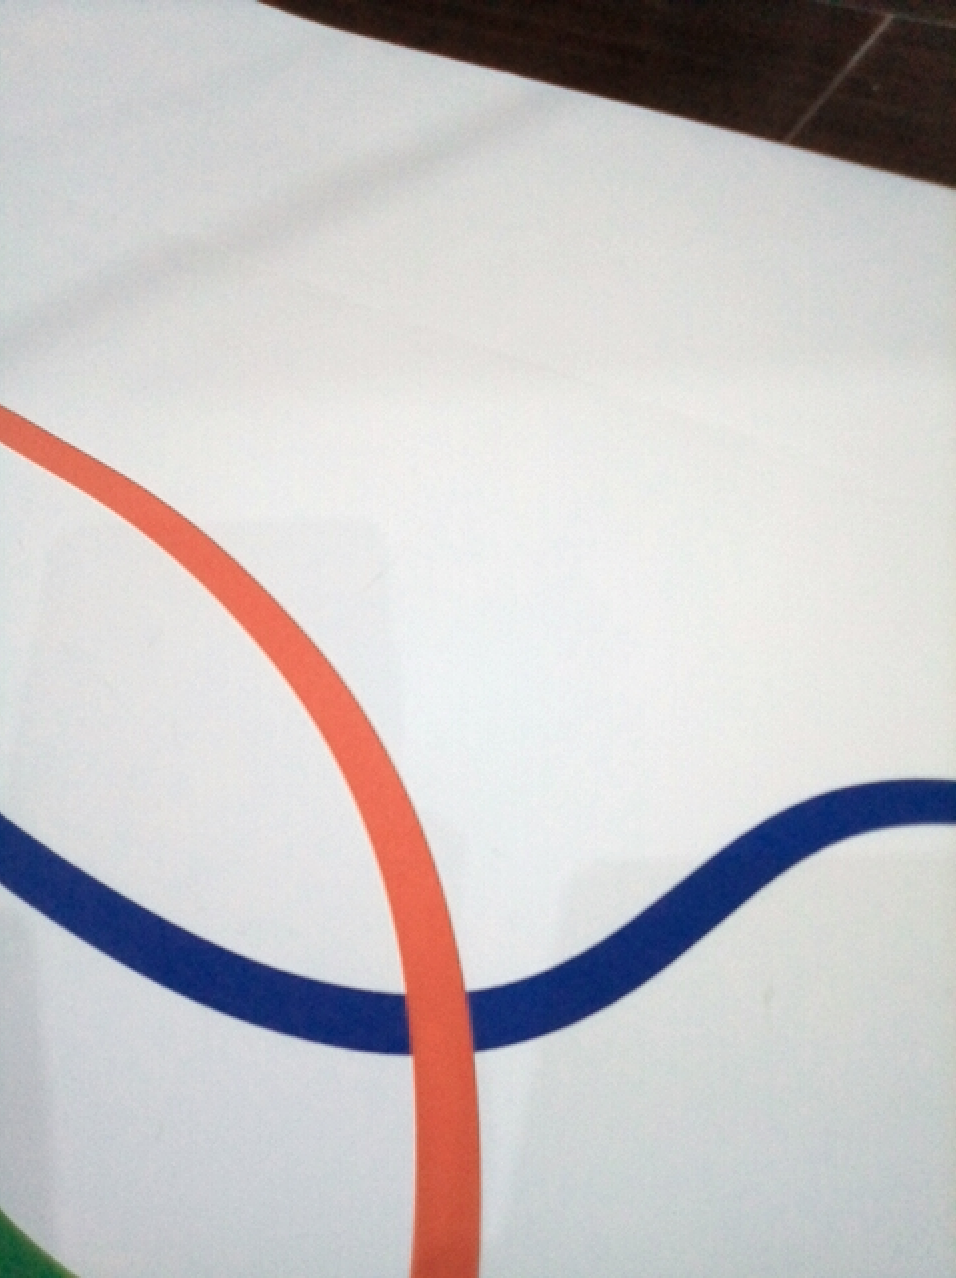
\includegraphics[scale=0.4]{img/image.png}
\caption{Camera image.}
\label{fig:image}
\end{figure}

First, a region of interest (ROI) is selected, as shown in Figure~\ref{fig:roi}. This is done in order to have better control over which part of the image is analyzed, allowing for faster processing and better error calculation. The way it was implemented, the user is allowed to select the relative distance of the top of the ROI to the top of the image. This is a floating point number between 0.0 and 0.8, where 0.0 represents the very top of the image and 0.8 the bottom, because the ROI height is fixed at 20\% of the image height.

\begin{figure}[thpb]
\centering
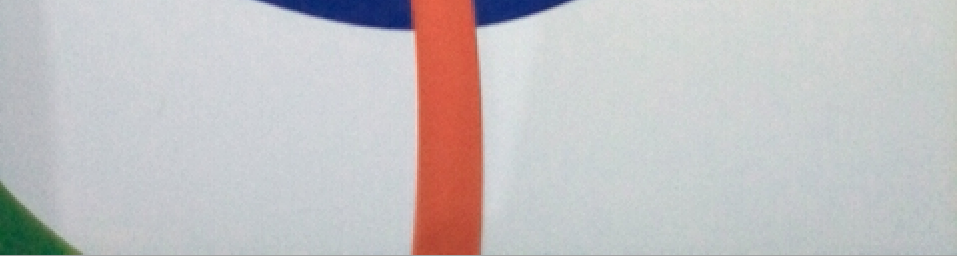
\includegraphics[scale=0.4]{img/roi.png}
\caption{ROI with red, blue and green lines.}
\label{fig:roi}
\end{figure}

Once the ROI is selected, a mask that detects only the desired color is computed. Then, the inverse of this mask is replaced by white, so that the only non white pixels are those belonging to the line, see Figure~\ref{fig:mask}.

\begin{figure}[thpb]
\centering
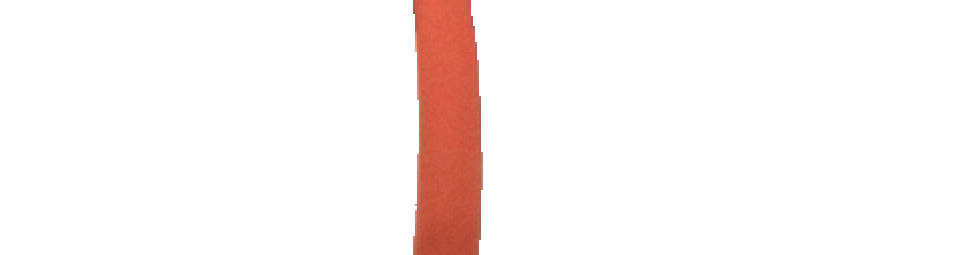
\includegraphics[scale=0.4]{img/mask.png}
\caption{ROI after mask with red line only.}
\label{fig:mask}
\end{figure}

This image is converted to gray scale, resulting in the image in Figure~\ref{fig:mono}, then it is blurred, see Figure~\ref{fig:blur}, and finally a threshold is computed, so that the line pixels become white and everything else is black, as in Figure~\ref{fig:thresh}

\begin{figure}[thpb]
\centering
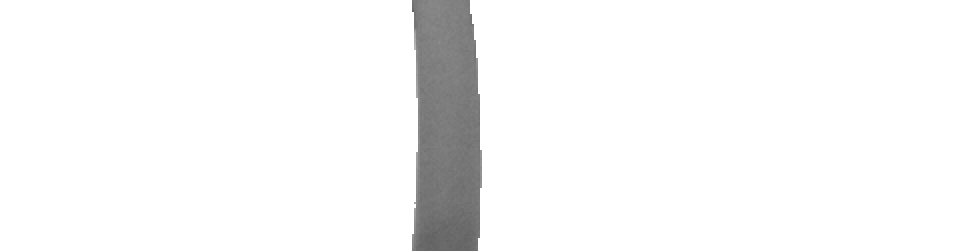
\includegraphics[scale=0.4]{img/mono.png}
\caption{Gray scale ROI with line.}
\label{fig:mono}
\end{figure}

\begin{figure}[thpb]
\centering
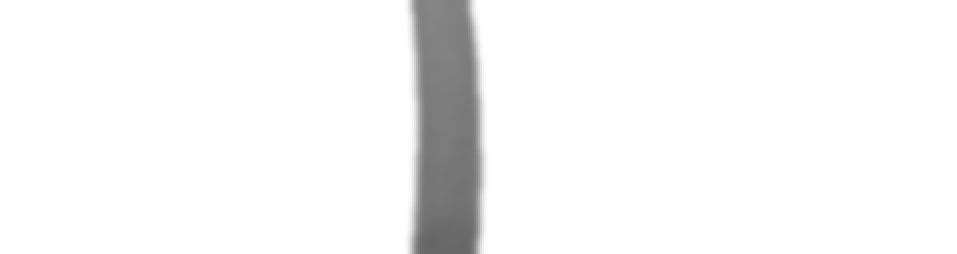
\includegraphics[scale=0.4]{img/blur.png}
\caption{Blurred ROI with line.}
\label{fig:blur}
\end{figure}

\begin{figure}[thpb!]
\centering
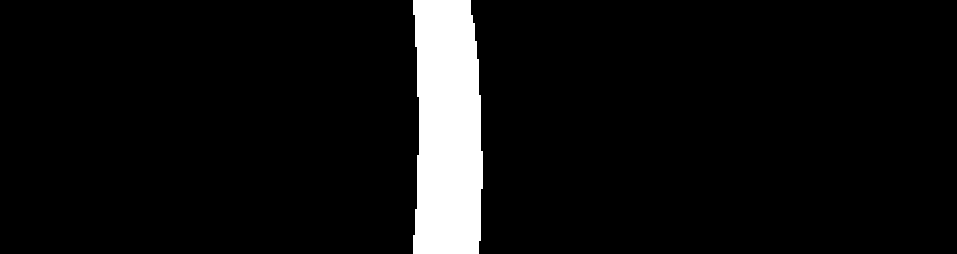
\includegraphics[scale=0.4]{img/thresh.png}
\caption{Thresholded ROI with line.}
\label{fig:thresh}
\end{figure}

In the final image processing steps, the contours of the image are computed, see Figure~\ref{fig:contour}. In most scenarios a single contour will be computed, or none, if there is no line of the chosen color in the ROI. But in order to account for those cases where two or more lines of the same color or two parts of the same line are visible in the ROI, the most central contour is selected. In fact, for each contour, its moments~\cite{moments_wiki} are computed and the centroid is then calculated as $$\left(\frac{m_{10}}{m_{00}}, \frac{m_{01}}{m_{00}}\right).$$ The minimum distance of the centroids to the center of the ROI determines which contour is selected. The error corresponding to that contour is then given by $$1 - 2 * \frac{m_{10}/m_{00}}{d},$$ where $d$ represents the width of the ROI. This yields a floating point number between -1 and 1, where -1 means the line is in the far right of the ROI, 1 means it is in the far left and 0 means it is in the middle.

\begin{figure}[thpb]
\centering
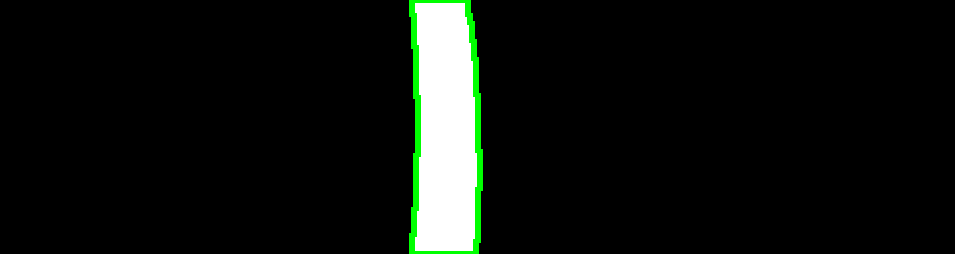
\includegraphics[scale=0.4]{img/contour.png}
\caption{ROI with line and contours.}
\label{fig:contour}
\end{figure}

Figure~\ref{fig:centroid} shows the ROI after threshold, with the line contours in green and the computed centroid in red. Since the line is slightly to the left of the center of the ROI, the corresponding error will be positive, but close to 0.

\begin{figure}[thpb]
\centering
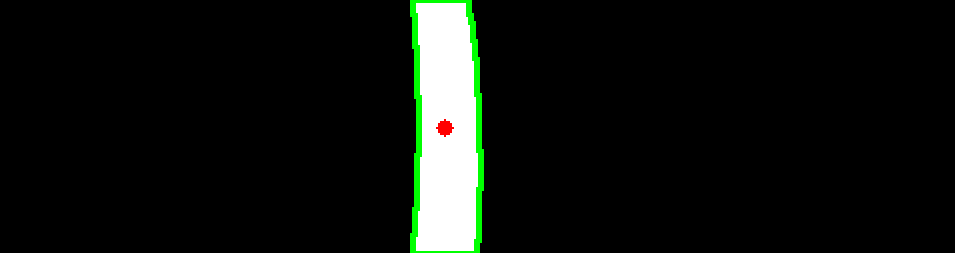
\includegraphics[scale=0.4]{img/centroid.png}
\caption{ROI with line, contours and centroid.}
\label{fig:centroid}
\end{figure}

\subsubsection{Initial random movement}

Until the first time a line is detected in the camera image from the phone, the robot will move randomly. The implementation of this random movement is very straightforward, a simple movement command is sent to the robot, setting the speed of each wheel to a random integer between 1 and 5. When the next camera image is received if the processing still fails to reveal a line to follow, a new random movement command is sent to the robot.

\subsubsection{Follow line movement}

After a line first is detected the robot will attempt move along following that line. To do this in a stable manner, a PID controller was implemented. The result is that at each image processed, the angular velocity of the robot is given by $$\omega = K_p * P + K_i * I + K_d * D,$$ where~$K_p, K_i$ and~$K_d$ are the proportional, integral and derivative constants defined by the user, and~$P, I$ and~$D$ are the proportional, integral and derivative terms, respectively. In this case,~$P = e$,~$I = I + e$ and~$D = e - d$, where~$e$ is the current error obtained from the image processing and~$d$ is the error obtained in the previous image. When the robot is initialized,~$e, d$ and~$I$ are all set to 0.

Since the velocity for each wheel must be specified in any move command, the final line following robot movement is given by setting the left wheel speed to~$v - \omega$ and the right wheel speed to~$v + \omega$, where~$v$ is the linear velocity defined by the user.

If at some point during its movement the robot loses sight of the line, that is, the ROI of the current image has no line of the desired color, then a new artificial error is computed as~$e = d / \abs{d},$ which means that the error is -1 if the previous error was negative and 1 if it was positive. Given that the robot just lost sight of the line, which we assume is continuous, the previous error should not be 0, but in the unlikely chance it is, then the current error is also set to 0. After this artificial error is computed, movement proceeds as usual.


%%%%%%%%%%%
% RESULTS %
%%%%%%%%%%%
\section{Results}

Since there is no simulator to test \robobo and the line following program, non virtual tests had to be conducted. For these tests the maps in Figures~\ref{fig:map_black} and~\ref{fig:map_color} where printed in large white paper and the robot was set up those maps, as shown in Figure~\ref{fig:map_color_robobo}.

\begin{figure}[thpb]
\centering
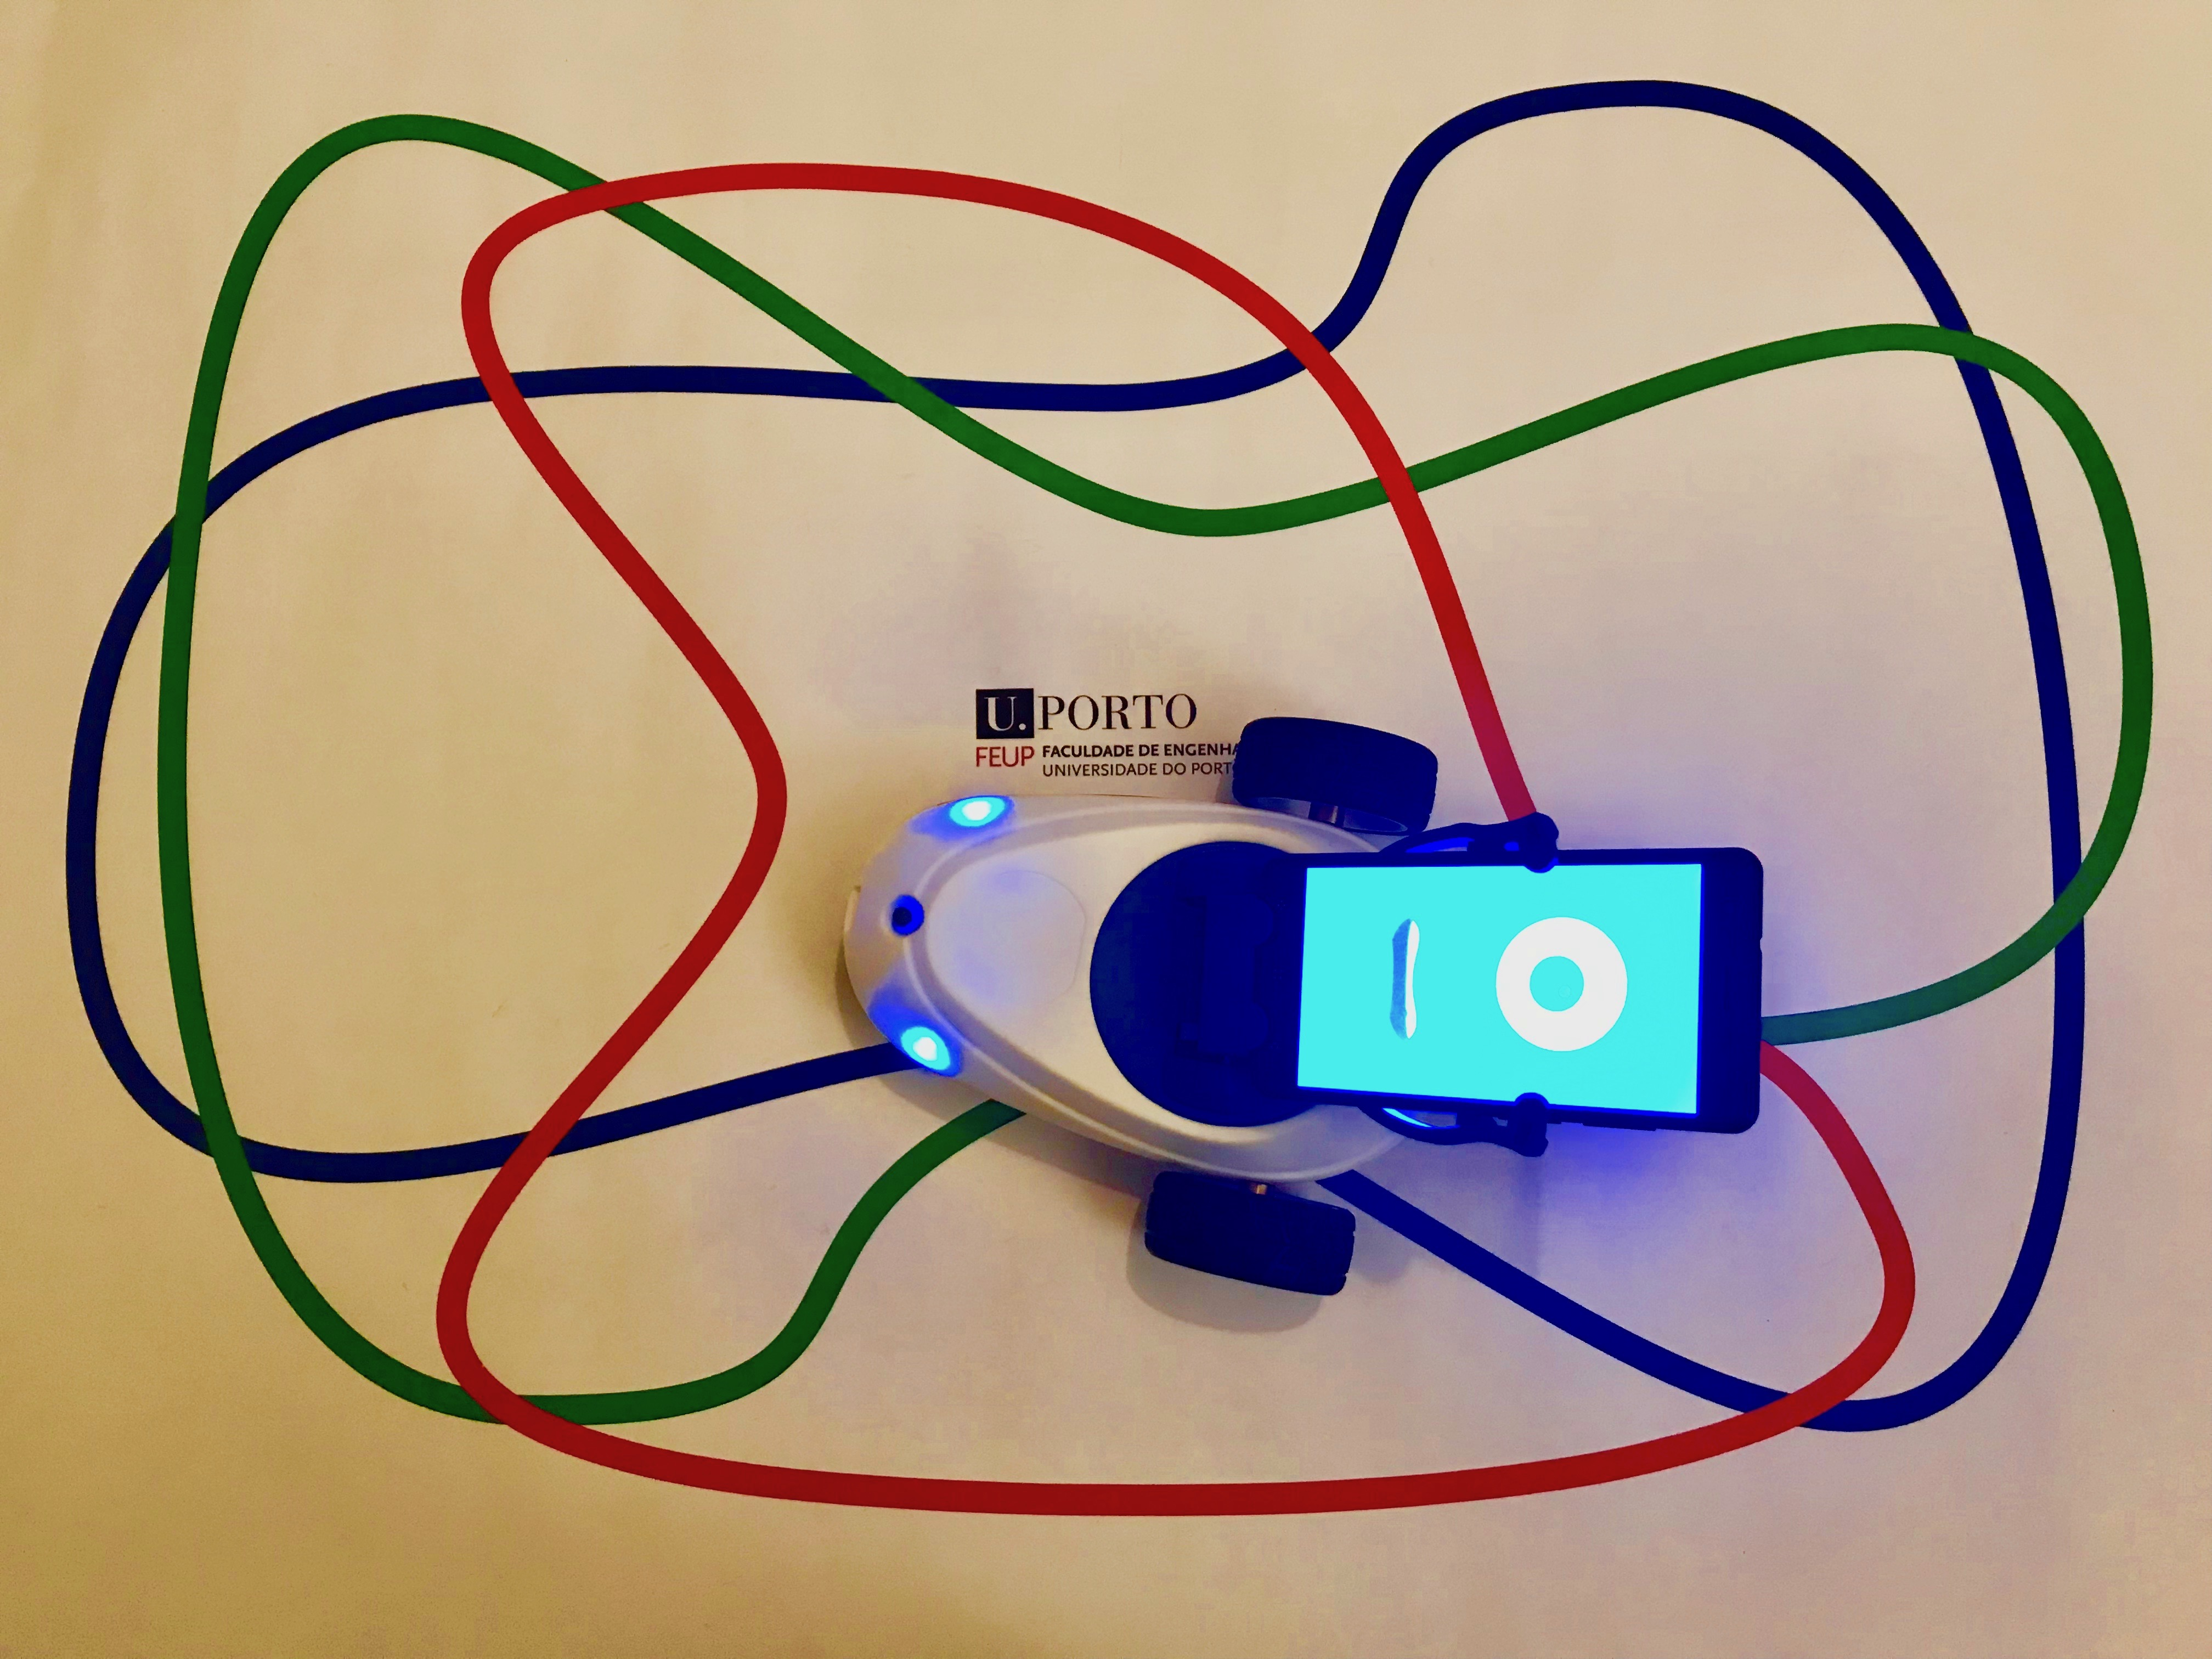
\includegraphics[scale=0.05]{img/map_color_robobo.jpg}
\caption{The colored lines map with \robobo.}
\label{fig:map_color_robobo}
\end{figure}

Because the random movement is not very relevant and is so simple, there is no real need to test it. Hence, for most tests, the robot was placed directly on top of the line it is supposed to follow. Also, in order to guarantee that the starting movements are simple, usually a straighter part of the line was chosen to place the robot.

\begin{figure}[thpb]
\centering
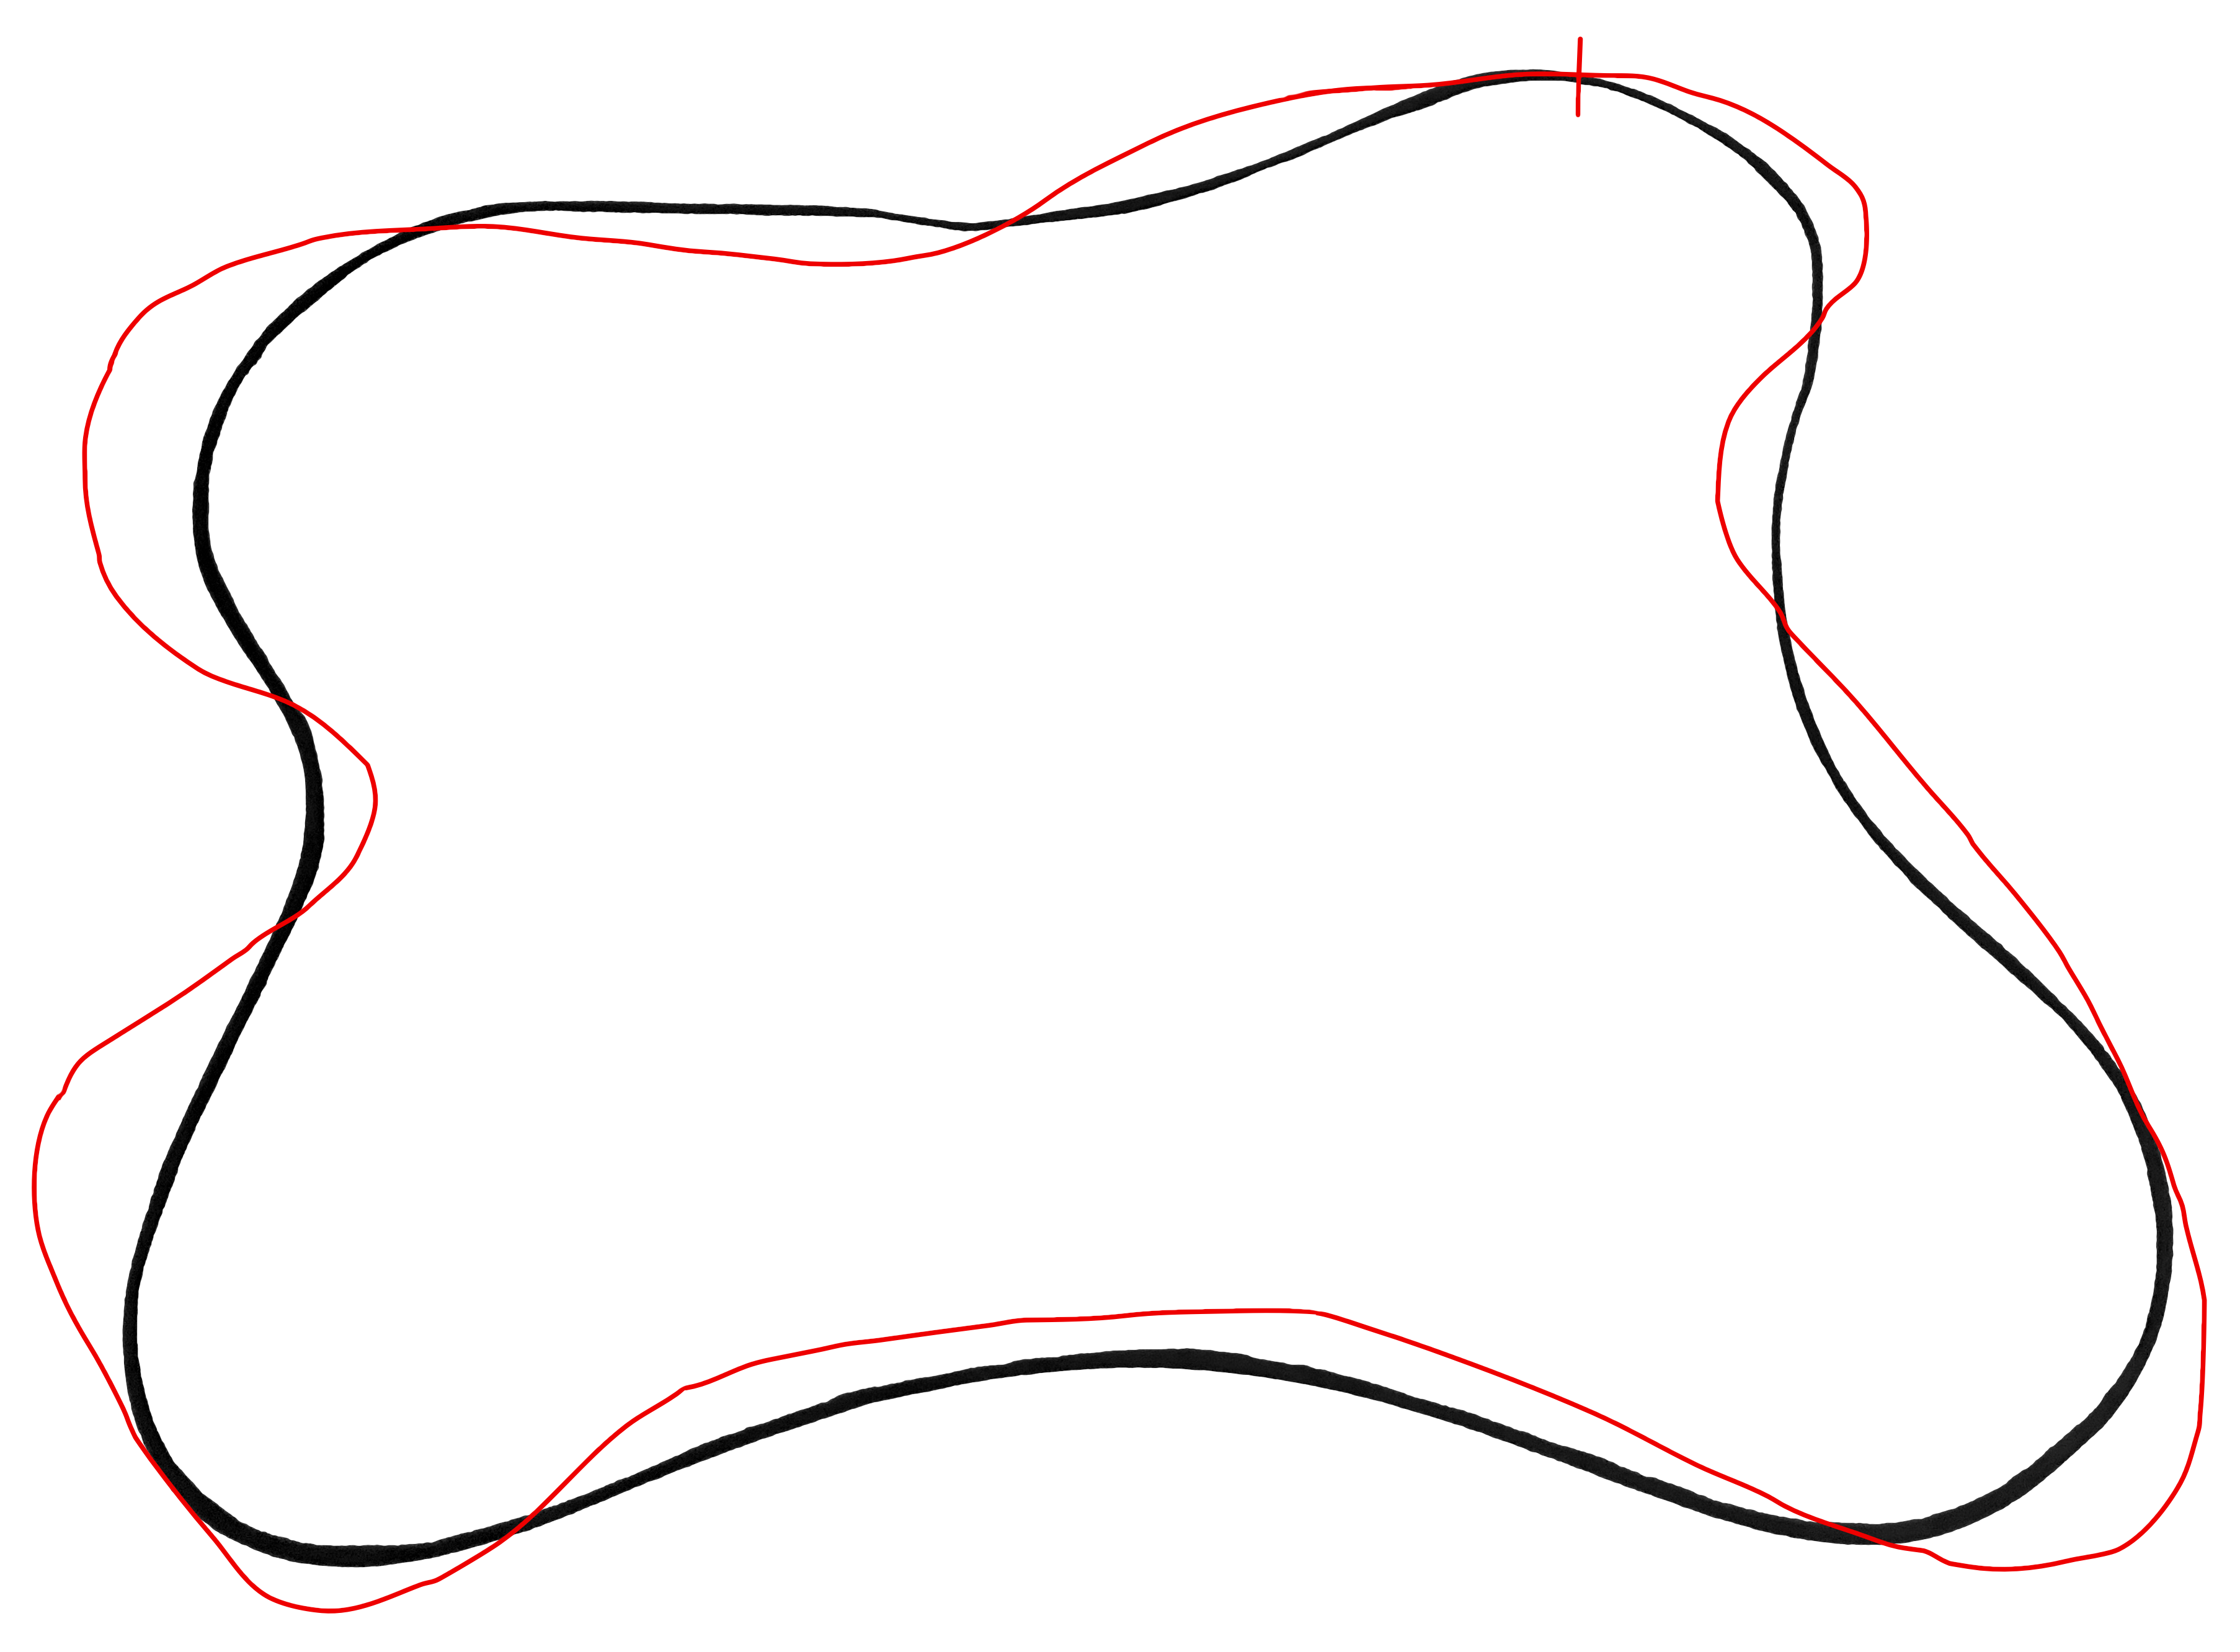
\includegraphics[scale=0.06]{img/result.png}
\caption{The black map and the line made by \robobo.}
\label{fig:result}
\end{figure}

In an attempt to measure both the stability of the robot and how closely it is able to follow the line, a pencil was attached to the front of the robot so that it could mark the passage of the robot through the map. The result of this experiment, which ran over the black line map, can be observed in Figure~\ref{fig:result}. The red line is the line made by \robobo while following the black line. The place where the robot was placed on the line is also marked.

The linear velocity for this test was 8, the distance of the ROI was 0.8 (closest to the robot) and the PID constants where~$K_p = 8, K_i = 0$ and~$K_d = 8$. As shown in Figure~\ref{fig:result}, with these parameters the movement of the robot is quite stable, in fact, there is practically no overreach followed by subsequent corrections. The red line does diverge from the original black line, especially in harder turns, but this is to be expected. In any case, better results can most likely be achieved with further tuning of the PID constants.

%%%%%%%%%%%%%%%
% LIMITATIONS %
%%%%%%%%%%%%%%%
\section{Limitations}

\subsection{Initial robot position}

If the robot is not properly placed on top of the line it should follow, then it may have trouble finding it. This happens when the random movement leads the robot to find the line in front of it but perpendicular to the robots orientation. In that case, the centroid of the contour of the line will be close to the center of the ROI, hence the computed error will be close to 0 and the robot will move forward, missing the line. Of course one could treat this special case separately in the image processing algorithm, but it would imply always testing for a case that should not happen once the robot starts following the line.

\subsection{Camera image width}

As mentioned above, placing the phone vertically, as the design of the Robobo implies, makes the camera image inadequate for line detection. The width of the image is simply too small, which makes the robot loose sight of the line every time it makes a semi-sharp turn.

In order to fix this, an artificial error is computed, which makes the robot turn harder in the direction it was already turning. In some cases this direction may be wrong, leading the robot to make a U-turn. Also, if the line is not spotted again, because the robot got to far away from it, the robot will just stay spinning circularly in the same spot.

\subsection{Linear velocity}

Due to the implementation of the \texttt{Robobo Developer} application, the camera image is already compressed when received in the line following program. This results in a very low quality image, especially if the robot is moving fast at the time the image is captured. Thus, faster linear velocities make the robot loose sight of the line more often and make its behavior more erratic, even after tunning the PID constants.

%%%%%%%%%%%%%%%
% CONCLUSION %
%%%%%%%%%%%%%%%
\section{Conclusion}

Although a line following robot is usually simple to implement, using the camera to sense the line poses a much more significant challenge, since it demands some knowledge of image processing. This was the most difficult, but also the most interesting and rewarding part of this project. 

Learning to deal with the frequent loss of the line also provided a good experience, once this limitation was accepted and appropriate measures to counter it where taken. Indeed, it was only after this implementation that the robot managed to take a full lap following the line without getting lost or completely ignoring some curves.

Also difficult, especially because there is no simulator, was tunning the PID constants. But unfortunately, apart from the moment where the robot actually started following the line in stable way, this part was quite boring.

The main objective of testing and learning to use \ros to program \robobo was clearly achieved. But the final resulting robot is also quite riveting, it is fun to see and hear the robot as it follows the line, temporarily losing track of it and going sad, then finding it again and going happy.

\section*{Acknowledgment}

The author would like to thank Fran Bellas, for technical help regarding \robobo as well as some hints on writing \texttt{C++} code, and Armando Sousa, for the colored map, an introduction to PID controllers and other advice.

%%%%%%%%%%%%%%%%
% BIBLIOGRAPHY %
%%%%%%%%%%%%%%%%
\bibliographystyle{IEEEtran}
\bibliography{IEEEabrv,line_bib}

\end{document}


